\documentclass[a4paper,10pt]{article}

\usepackage{graphicx}  
\usepackage{libertine}%  serif and sans serif
\usepackage[scaled=0.85]{beramono}%% mono
\usepackage{titlesec}
\usepackage[utf8]{inputenc}
\usepackage[normalem]{ulem}
\usepackage[usenames,dvipsnames]{color}
\usepackage{bbm}
\usepackage{bm}
\usepackage{flafter}	% keine Gleitobjekte vor der Position, an der sie definiert werden
\usepackage{color}
\usepackage[font=small,labelfont=bf,format=hang]{caption}[2017/02/28]		% Bildlegenden etc. anpassen
\usepackage{subfigure}		% für subfigures
\usepackage{pdfsync}	% erste llt Sync Datei für Sumatra Pdf Reader
\usepackage{array}
\usepackage{tabularx} 
\usepackage{longtable}	% kann Seitenumbrüche auch bei Tabellen
\usepackage{url}
\usepackage[a4paper,width=150mm,top=15mm,bottom=10mm]{geometry}

\setlength{\textwidth}{15cm}

\setlength{\headheight}{10pt}
\setcounter{secnumdepth}{3}
\setcounter{tocdepth}{3}

\sloppy 

%--------------------BEGIN DOCUMENT----------------------
\begin{document}

%--------------------TITLE-------------
\noindent\begin{minipage}{0.4\textwidth}% adapt widths of minipages to your needs
\par{
		{\Huge Sergey Platonov
	}\bigskip\par} 
%Place and Date of Birth: Mogilev, Belarus  | 29 July 1988 \\
\end{minipage}%
\hfill%
\begin{minipage}{0.35\textwidth}
\vspace{0.2cm}
\begin{doublespacing}
Address:    Schlo{\ss}str. 33, 10459, Berlin \\
Phone:    (+49)-176-8333-26-53\\
Email:     {platonov.serge@gmail.com}
LinkedIn: serge-platonov-06711a136
Facebook: siarhei.platonau
\end{doublespacing}
\end{minipage}%
\hfill%
\begin{minipage}{0.2\textwidth}\raggedleft
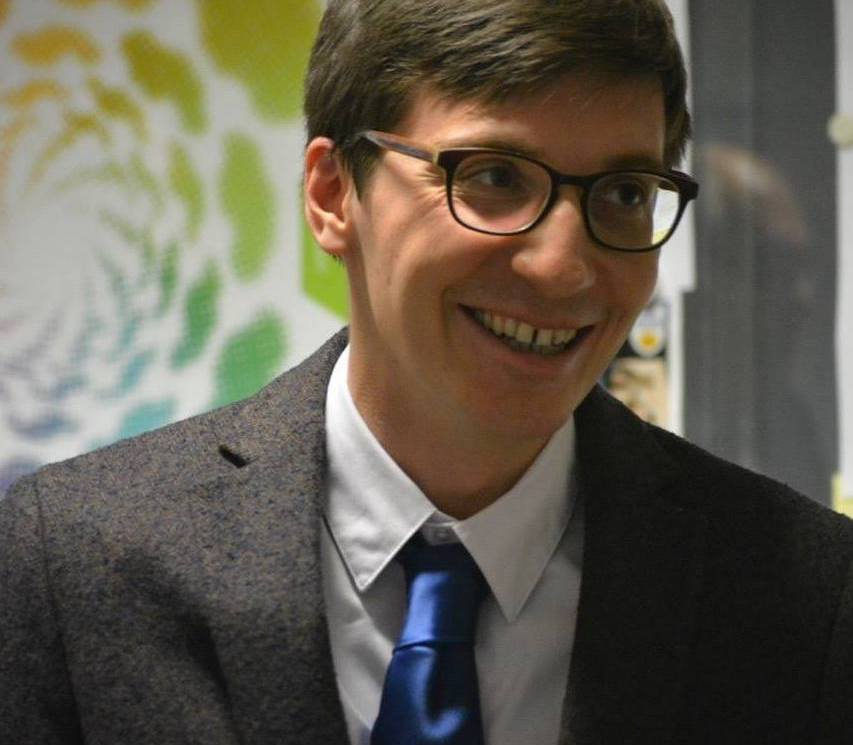
\includegraphics[width=1\textwidth]{1.jpg}
\end{minipage}
%\hfill%
%--------------------SECTIONS-----------------------------------
%----------------------------------------------------------------------------------------
%	Abstract SECTION
%----------------------------------------------------------------------------------------
\section*{}
\vspace{-1cm}
\text
I am a \textbf{project manager} with experience in solving \textbf{engineering problems} and the \textbf{data analysis} tasks. My academic training, the ability of \textbf{strategic planning} and strong \textbf{information and time management} prepare me to be an effective part of the company team.}

%----------------------------------------------------------------------------------------
%	WORK EXPERIENCE SECTION
%----------------------------------------------------------------------------------------
%\section*{Education}
%\begin{flushleft}{2012-current}\hfill PhD in Physics \hfill  \textbf{Ludwig-Maximilians University, Munich}\end{flushleft}
%\begin{flushleft}{2010-2012}\hfill M.Sc. with Honours \hfill  \textbf{Moscow Institute of Physics and
%Technology}\hfillGPA = 4.87 out of 5 \end{flushleft}
%\begin{flushleft}{2006-2010}\hfill B.Sc. with Honours \hfill  \textbf{Moscow Institute of Physics and
%Technology}\hfillGPA = 4.92 out of 5 \end{flushleft}
%----------------------------------------------------------------------------------------
%	TECHNICAL STRENGTHS SECTION
%----------------------------------------------------------------------------------------

\section*{Work Experience}
\begin{flushleft}{\textbf{PhD Researcher|Project Manager}, \textbf{Paul-Drude-Institut, Berlin, \text{2015 – 2017}}\end{flushleft}
\begin{itemize}
\item Organizing the relocation of the physics lab consisting of more than $1000$ units from Munich to Berlin and installing it on the new location.
\item Technical management for choosing and ordering the new EBL system with budget of $1$ million €\
\item Handling the measurement data (2D arrays of $\propto3000$ elements) including visualisation, data organizing and fitting.
\item Statistical analysis of the data: FFT, wavelet transform, fractal dimension analysis. 
\item Preparation and publishing $3$ scientific papers and more than $5$ conference applications and reports.
\item Improving and automatisation the measurement software and implementing new devices into the measurement framework of more than $100$ devices.
\end{itemize}

\begin{flushleft}\textbf{PhD Researcher|Project Manager}, \textbf{Ludwig-Maximilians-Universit{\"a}t, Munich, {\text{2012 – 2015}}}\end{flushleft}
\begin{itemize}
\item Supervising the work of $2$ master and one bachelor student.
\item Budget management of around $30000\,$€, ordering of supplies and expensive measurement devices.
\item Engineering seminconductor samples with characteristic sizes of $\proprto 100\,$nm in the clean room 
by optical lithography and electron-beam lithography.
\item Designing the circuit boards including RF filtering and attenuation in the limited cryogenic conditions (sizes $<5\times5\times5\,$cm).
\item Electrical characterization of the samples by radio-frequency below $20\,$GHz and DC methods with sensitivity below $1$pA at cryogenic temperatures.
%\item Testing and characterization of cryogenic equipment: dilution fridges, He$^3$ systems, superconducting magnets.
%\item Leak testing of the vacuum systems including rotary/turbo/diffusion pumps.
\item Teaching assistance at the lab-course “Thermoelectrics” for 5th-6th semester master students and exercises for the lecture “Advanced Solid State Physics” by Prof. Alex H\"ogele.
\end{itemize}

\begin{flushleft}{\textbf{Project Engineer}, \textbf{Institute of Radioelectronics and Engineering, Moscow, \text{2009 – 2012}}}
\end{flushleft}
\begin{itemize}
\item Budget management of $1$ million rubles, ordering of supplies and measurement devices.
\item Developing the simulation software for wave propagation in multilayered magnetic/acoustic structures.
\item Participation in $11$ conferences and collaboration in the international project of OOMMF simulation.
\item Section secretary of $3$ MIPT scientific conferences.
\end{itemize}

%----------------------------------------------------------------------------------------
%	EDUCATION SECTION
%----------------------------------------------------------------------------------------
\section*{Education}
\begin{tabular}{llll}
2012-2017 & Dr. rer. nat. & Ludwig-Maximilians-Universit{\"a}t & Cum Laude 1.6  \\ 
2010-2012 &  M.Sc. with Honours & Moscow Institute of Physics and
Technology & GPA = 4.87 out of 5\\
2006-2010 & B.Sc. with Honours & Moscow Institute of Physics and
Technology &  GPA = 4.92 out of 5\\
\end{tabular}
%----------------------------------------------------------------------------------------
%	LanguagesG
%----------------------------------------------------------------------------------------
\section*{Languages} 
\begin{itemize}
\item Belarussian, Russian | native language
\item English | full working proficiency (C1)
\item German | full working proficiency (C1)
\end{itemize}
%----------------------------------------------------------------------------------------
%	Software
%----------------------------------------------------------------------------------------
\section*{Software}
\begin{tabular}{l|l|l}
Programming languages & Labview  & Expert\\
 & C/C++ & Good  \\ 
 & Python  & Expert\\
 & SQL  & Basic\\
\hline
Data analysis & Matlab  & Expert\\
 & Maple & Good  \\ 
 & Mathcad  & Expert\\
 & Mathematica  & Good\\
  & SPSS  & Basic\\
\hline
Python libraries & Matplotlib  & Expert\\
 & Scipy & Expert  \\ 
 & Numpy  & Expert\\
 & Scikit  & Good\\
 & Pandas  & Good\\
\hline
CAD & Solidworks  & Expert\\
 & AutoCad & Basic  \\ 
 & Eagle  & Expert\\
 & P-Cad  & Good\\
\hline
Text organizing tools & Latex  & Expert\\
 & MS Office & Expert  \\ 

\end{tabular}
%\begin{itemize}
%\item Programming languages : C/C++ \\, Python\\, SQL\\Researcher|.
%\item Data analysis: Matlab, Maple, Mathcad, Mathematica, Python based: Matplotlib, Scipy, Numpy. 
%\item Simulation frameworks: Sonnet, Kwant, OOMMF, COMSOL, Agros2D.
%\item Technical drawings: Solidworks, AutoCad, Eagle.
%\item Text processing and organizing: Latex, MS Powerpoint, MS Excel, MS Word, MS Access.
%\end{itemize}

%----------------------------------------------------------------------------------------
%	Academic Achievementss
%----------------------------------------------------------------------------------------
%\clearpage

\section*{Academic Achievements} 
\begin{itemize}
\item Fellowship of Foundation of non-commercial Programs “Dynasty” for students, 2011-2012
\item Winner of the research works contest on 54th MIPT scientific conference, 2011
\item Candidate to Belarus team on International Physics Olimpiad (IPho) in Singapore, 2006
\end{itemize}
%----------------------------------------------------------------------------------------
%	Publications
%----------------------------------------------------------------------------------------

%Hobbies

\section*{Hobbies/Interests} 

Intellectual quizzes, hiking, badmintion, board games, data challenges on kaggle.com.

%	EXAMPLE SECTION
%----------------------------------------------------------------------------------------


%\section*{Selected publications}

%\begin{itemize}
%\item \textit{Mesoscopic Field-Effect-Induced Devices in Depleted Two-Dimensional Electron Systems}, Phys. Rev. Applied 8, 064015, December 14, 2017
%\item \textit{Gaussian Beam Electron Optics with Quantum Point Contacts}, German-Japanese Meeting on the Science of Hybrid Quantum Systems , Berlin, 10-11 November 2016
%\item \textit{Lissajous Rocking Ratchet: Realization in a Semiconductor Quantum Dot}, Phys. Rev. Lett. 115, 106801, 2015
%\item \textit{Anomalous Hall effect in magnonic crystals}, Book of Abstract Advanced Electromagnetic  Symposium “AES 2012”, Paris, April 16- 19, 2012
%\item \textit{Magnetostatic spin waves propagation in two-dimensional wedge magnonic crystal}, Book of Abstract European Conference “PHYSICS OF MAGNETISM”, Poznan, Poland, June 27- July 1, 2011
%\end{itemize}

%----------------------------------------------------------------------------------------
%\begin{section}{Relevant Courses}
%todo

%\end{section}
%\newpage
%\hypertarget{gmat}{\textsc{Gmat}\setmainfont{LMRoman10 Regular}\textregistered\setmainfont[SmallCapsFont=Fontin-SmallCaps]{Fontin-Regular}}

%\XeTeXpdffile ''GMAT.pdf'' page 1 scaled 800

\end{document}
